\documentclass[landscape]{jhuslides3C}
\usepackage{url}
\usepackage{amsmath}
\usepackage{graphicx}
\usepackage{color}
\usepackage{colortbl}
%\usepackage{epic,ecltree}
%\usepackage{bar}
%\usepackage{qtree}
%\usepackage{eclbip}
\usepackage{fancybox}
\usepackage{pause} % java -jar ~/Code/bin/pp4p.jar mtsummit09-talk.pdf mtsummit09-talk.view.pdf
\usepackage[absolute]{textpos}
\pdfoptionpdfminorversion 3
%\usepackage{courier}
\usepackage{tikz}
%\usepackage{tikz-qtree}
\usetikzlibrary{calc,matrix}
%\usepackage{algorithmic}
%\usepackage{algorithm}
\usepackage{amssymb,latexsym} % for \blacklozenge
%\renewcommand{\algorithmicrequire}{\textbf{Input:}}
%\renewcommand{\algorithmicensure}{\textbf{Output:}}
%\renewcommand{\algorithmiccomment}[1]{// {\em #1}}
\usepackage{multicol}
\usepackage{wasysym} % smileys
\renewcommand*\ttdefault{txtt} % 20% tighter than courier
\usepackage{hyperref}

\definecolor{lightblue}{rgb}{.8,.8,1}
\definecolor{mediumlightblue}{rgb}{.5,.5,1}
\definecolor{lightyellow}{rgb}{1,1,.5}
\definecolor{lightorange}{rgb}{1,.9,.7}
\definecolor{darkorange}{rgb}{1,.75,.2}
\definecolor{sortadarkorange}{rgb}{.8,.5,.1}
\definecolor{verydarkorange}{rgb}{.5,.3,0}
\definecolor{darkblue}{rgb}{0,0,0.8}
\definecolor{verydarkgreen}{rgb}{0,0.4,0}
\definecolor{darkgreen}{rgb}{0,0.8,0}
\definecolor{darkred}{rgb}{0.8,0,0}
\definecolor{verydarkred}{rgb}{0.6,0,0}
\definecolor{lightgreen}{rgb}{.8,1,.8}
\definecolor{lightred}{rgb}{1,.8,.8}
\definecolor{darkgrey}{rgb}{0.5,0.5,0.5}
\definecolor{purple}{rgb}{0.6,0,0.6}
\definecolor{red}{rgb}{1,0,0}
\definecolor{orange}{rgb}{.8,.6,0}
\definecolor{cyan}{rgb}{0,.6,.6}
\definecolor{reddishgreen}{rgb}{0.4,0.6,0}

\newcommand{\newconcept}[1]{\textcolor{blue}\textbf{#1}}
\newcommand{\example}[1]{\textcolor{darkblue}{\rm #1}}
\newcommand{\important}[1]{\textcolor{darkblue}{\em #1}}
\newcommand{\concept}[1]{\textcolor{darkblue}{\em #1}}
\newcommand{\maths}[1]{\textcolor{purple}{#1}}
\newcommand{\mathstt}[1]{\textcolor{purple}{$\mathtt{#1}$}}
\newcommand{\reference}[1]{\vspace{-2mm}\begin{flushright}\textcolor{purple}{\tiny [from #1]}\end{flushright}\vspace{-7mm}}
\renewcommand{\url}[1]{\textcolor{verydarkred}{\tt #1}}

\newcommand{\highlightbox}[6]{\begin{textblock}{#3}(#1,#2) \colorbox{#4}{\textcolor{#5}{\begin{minipage}{#3in} #6 \end{minipage} }} \end{textblock}}
\newcommand{\backgroundbox}[5]{\highlightbox{#1}{#2}{#3}{#5}{black}{\vspace{#4in}\hspace{#3in}}}
\newcommand{\currenttopic}[1]{\colorbox{lightyellow}{\textcolor{black}\textbf{#1}}}

\newcommand{\littlecode}[1]{\colorbox{gray}{\textcolor{black}{\small \tt #1}}}
\newcommand{\highlight}[1]{\colorbox{lightyellow}{#1}}
\newcommand{\highlightOrange}[1]{\colorbox{lightorange}{#1}}
\newcommand{\highlightGreen}[1]{\colorbox{lightgreen}{#1}}
\newcommand{\highlightBlue}[1]{\colorbox{lightblue}{#1}}

\usepackage{palatino}

%%%%%%%%%%%%%%%%%%%%%%%%%%%%%%%%%%%%%%%%%%%%%%%%%%%%%%%%%%%%%%%%%%%%%%%%%%%%

\begin{document}\rm
\title[Introduction to Human Language Technology: Introduction]{Introduction to Human Language Technology}
\author[Philipp Koehn]{Philipp Koehn}
\date{31 August 2021}
\maketitle

%%%%%%%%%%%%%%%%%%%%%%%%%%%%%%%%%%%%%%%%%%%%%%%%%%%%%%%%%%%%%%%%%%%%%%%%%%%%

\slide{Administrative}
\vfill
\begin{itemize} \itemsep 0mm
\item \textbf{Coordinator:} Philipp Koehn (phi@jhu.edu)
\item \textbf{Lecturers:} Faculty of the Center for Language and Speech Processing (CLSP)
\item \textbf{TA:} Suzanna Sia (ssia1@jhu.edu)
\item \textbf{Class:} Monday, Wednesday, 9:00-10:15pm, Ames 234
\item \textbf{Course web site:} \href{https://jhu-intro-hlt.github.io/}{\tt https://jhu-intro-hlt.github.io/}
\item \textbf{Grading} \vspace{-3mm}
\begin{itemize}
\item 5 assignments (10\% each)
\item first midterm exam (15\%)
\item second midterm exam (15\%)
\item final exam (20\%)
\end{itemize}
\end{itemize}
\vfill

%%%%%%%%%%%%%%%%%%%%%%%%%%%%%%%%%%%%%%%%%%%%%%%%%%%%%%%%%%%%%%%%%%%%%%%%%%%%

\slide{Course Overview}
\vfill
\begin{itemize}
\item Human Language Technology
\begin{itemize}
\item Speech: spoken language (audio)
\item Text: written language (text)
\end{itemize}
\item Means of Communication\\
$\rightarrow$ new ways of interacting with computers
\item Storage medium for knowledge\\
$\rightarrow$ new ways of making word knowledge available
\item This course
\begin{itemize}
\item methods and tools used in HLT
\item overview of HLT applications
\end{itemize}
\end{itemize}
\vfill


%%%%%%%%%%%%%%%%%%%%%%%%%%%%%%%%%%%%%%%%%%%%%%%%%%%%%%%%%%%%%%%%%%%%%%%%%%%%

\slide{Course Overview: Text}
\vfill
\begin{itemize} \itemsep 0mm
\item Words, Morphology (Yarowsky)
\item Syntax (Post)
\item Semantics (Lippincott, Koehn)
\item Deep Learning (Murray)
%\item Outsourcing linguistic data annotation
\item Information retrieval and extraction (Koehn, Duh)
\item Machine translation (Murray)
\end{itemize}
\vfill



%%%%%%%%%%%%%%%%%%%%%%%%%%%%%%%%%%%%%%%%%%%%%%%%%%%%%%%%%%%%%%%%%%%%%%%%%%%%

\slide{Course Overview: Speech}
\vfill
\begin{itemize} \itemsep 0mm
\item Audio signals, phonemes, graphemes, dictionaries (Elhilali)
\item Auditory system (TBD)
\item Signal processing (Khudanpur)
\item Speech recognition: HMM (Khudanpur)
\item End-to-end neural speech recognition (TBD) 
\item Speaker identification, language identification (Dehak)
\end{itemize}
\vfill

%%%%%%%%%%%%%%%%%%%%%%%%%%%%%%%%%%%%%%%%%%%%%%%%%%%%%%%%%%%%%%%%%%%%%%%%%%%%

\slide{Course Overview: Applications}
\vfill
\begin{itemize} \itemsep 0mm
\item NLP for Digital Humanities (Lippincott)
\item Question answering (Duh)
\item Dialog systems (TBD)
\item Clinical NLP (Dredze)
\item Ethical problems (Moro-Velazquez)
\item Analyzing and Interpreting Neural Networks for NLP (TBD)
\end{itemize}
\vfill

%%%%%%%%%%%%%%%%%%%%%%%%%%%%%%%%%%%%%%%%%%%%%%%%%%%%%%%%%%%%%%%%%%%%%%%%%%%%

\slide{Master Concentration in HLT}
\vfill
\begin{center}
\tt https://www.clsp.jhu.edu/human-language-technology-masters/
\end{center}
%\vfill
\begin{itemize}
\item New this year: Concentration in Human Language Technology
\begin{itemize}
\item Master in Computer Science
\item Master in Electrical and Computer Engineering
\end{itemize}
\item Requirements (in addition to usual degree requirements)
\begin{itemize}
\item Introduction to Human Language Technology (601.667)
\item Natural Language Processing (601.665)
\item Information Extraction from Speech and Text (520.666)
\item Master project in HLT
\end{itemize}
%\item Application forms at the end of this semester (including project selection)
\end{itemize}
\vfill

%%%%%%%%%%%%%%%%%%%%%%%%%%%%%%%%%%%%%%%%%%%%%%%%%%%%%%%%%%%%%%%%%%%%%%%%%%%%

\slide{Center for Language and Speech Processing}
\vfill
\begin{itemize}
\item One of the largest and most influential academic research centers in HLT
\item Faculty in Computer Science, Electrical and Computer Engineering, Cognitive Science, Mathematical Sciences, ...
\item Home of over 60 researchers, dozens of PhD students
\item Founded in 1992 by Frederick Jelinek (1932-2010)
\item Sibling center: Human Language Technology Center of Excellence (HLTCOE)
\end{itemize}
\vfill

%%%%%%%%%%%%%%%%%%%%%%%%%%%%%%%%%%%%%%%%%%%%%%%%%%%%%%%%%%%%%%%%%%%%%%%%%%%%

\slide{Speech Recognition}
\vfill
\begin{center}
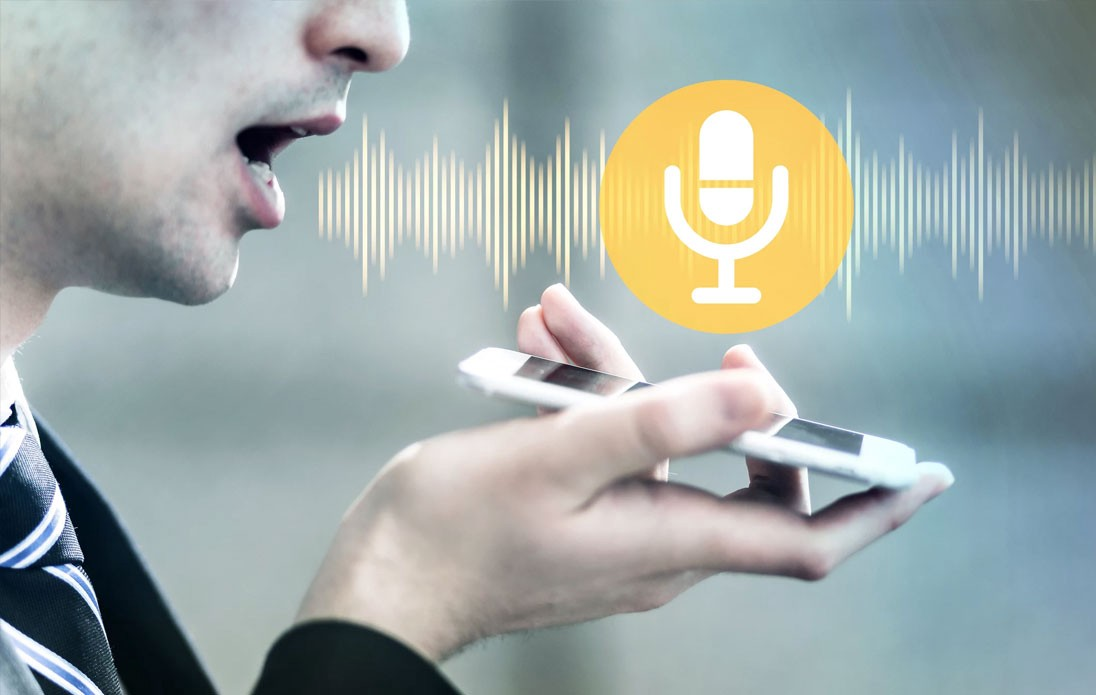
\includegraphics[width=23cm]{speech-recognition.jpg}
\end{center}
\vfill

%%%%%%%%%%%%%%%%%%%%%%%%%%%%%%%%%%%%%%%%%%%%%%%%%%%%%%%%%%%%%%%%%%%%%%%%%%%%

\slide{Information Retrieval}
\vfill
\begin{center}

\includegraphics[width=20cm]{information-retrieval1.png}\\

\includegraphics[width=20cm]{information-retrieval2.png}\\
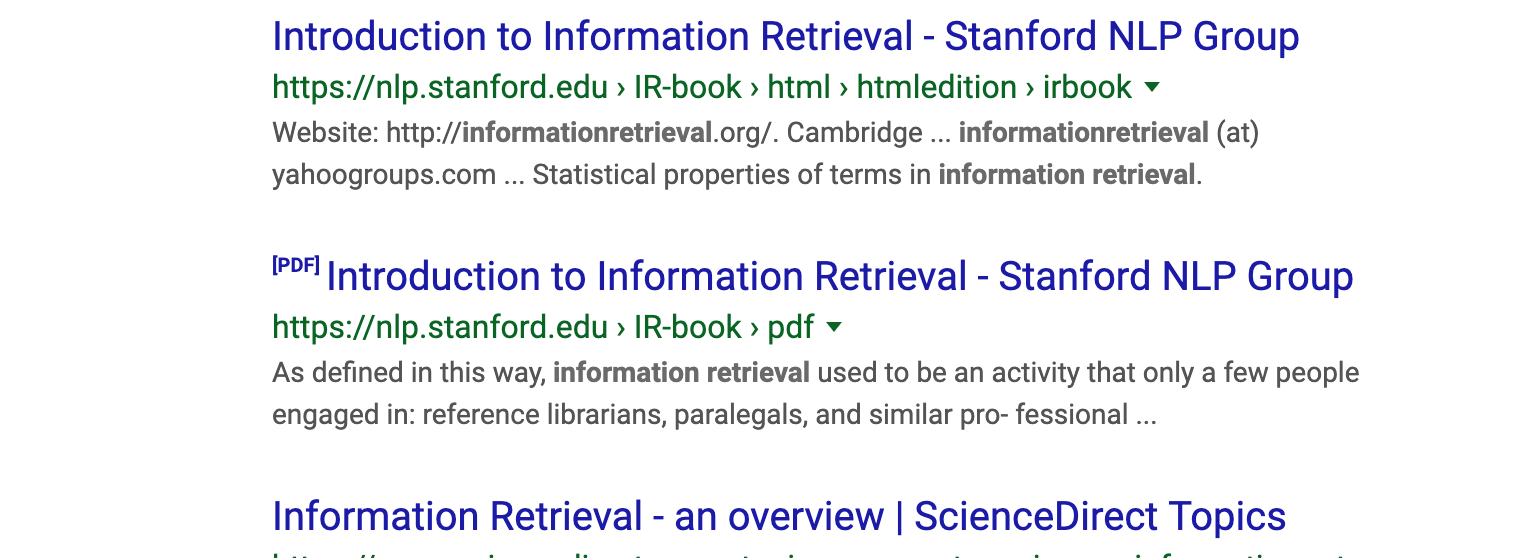
\includegraphics[width=20cm]{information-retrieval3.png}
\end{center}
\vfill

%%%%%%%%%%%%%%%%%%%%%%%%%%%%%%%%%%%%%%%%%%%%%%%%%%%%%%%%%%%%%%%%%%%%%%%%%%%%

\slide{Information Extraction}
\vfill
\begin{center}
\includegraphics[width=20cm]{information-extraction.png}
\end{center}
\vfill

%%%%%%%%%%%%%%%%%%%%%%%%%%%%%%%%%%%%%%%%%%%%%%%%%%%%%%%%%%%%%%%%%%%%%%%%%%%%

\slide{Machine Translation}
\vfill
\begin{center}
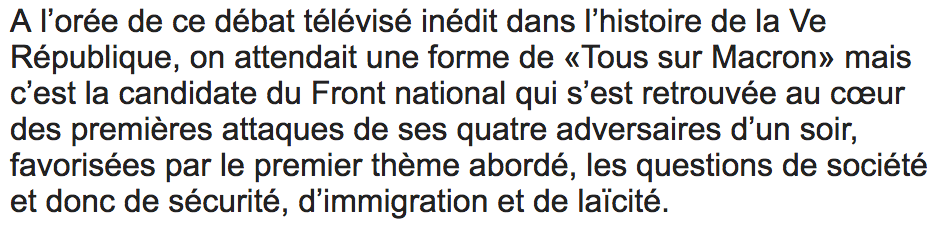
\includegraphics[width=27cm]{google-translate-mar2017-french-source.png}

\vspace{10mm}
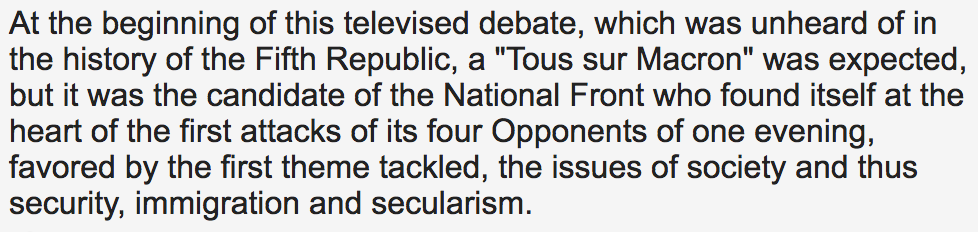
\includegraphics[width=27cm]{google-translate-mar2017-french-target.png}
\end{center}
\vfill

%%%%%%%%%%%%%%%%%%%%%%%%%%%%%%%%%%%%%%%%%%%%%%%%%%%%%%%%%%%%%%%%%%%%%%%%%%%%

\slide{Question Answering}
\vfill
\begin{center}
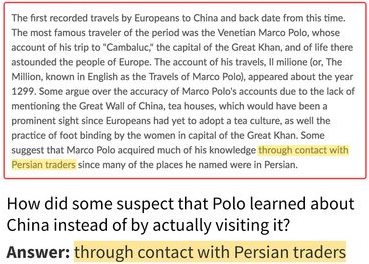
\includegraphics[width=20cm]{question-answering.jpeg}
\end{center}
\vfill

%%%%%%%%%%%%%%%%%%%%%%%%%%%%%%%%%%%%%%%%%%%%%%%%%%%%%%%%%%%%%%%%%%%%%%%%%%%%

\slide{Dialog Systems}
\vfill
\begin{center}
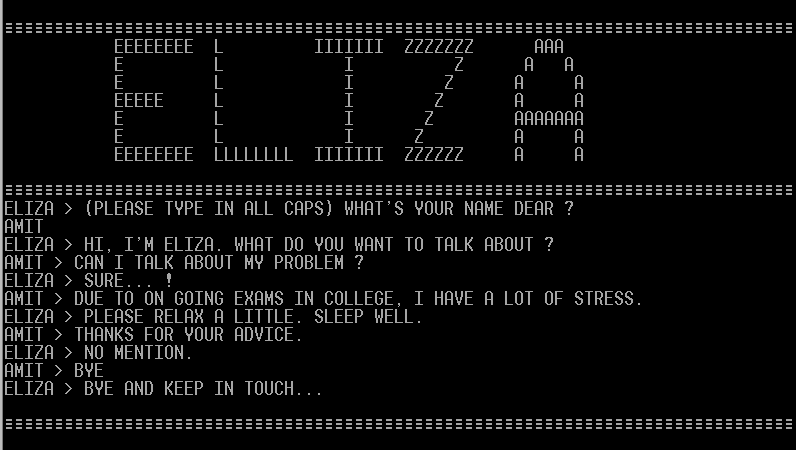
\includegraphics[width=25cm]{eliza.png}
\end{center}
\vfill

%%%%%%%%%%%%%%%%%%%%%%%%%%%%%%%%%%%%%%%%%%%%%%%%%%%%%%%%%%%%%%%%%%%%%%%%%%%%

\slide{Call Center}
\vfill
\begin{center}
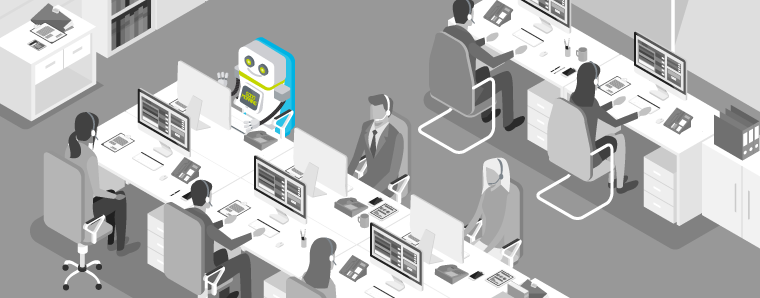
\includegraphics[width=25cm]{CallCenterAutomation.png}
\end{center}
\vfill


%%%%%%%%%%%%%%%%%%%%%%%%%%%%%%%%%%%%%%%%%%%%%%%%%%%%%%%%%%%%%%%%%%%%%%%%%%%%

\slide{Hate Speech Detection}
\vfill
\begin{center}

\includegraphics[width=20cm]{hate-speech.png}\\[1cm]
incitement of violence / dehumanizing individuals or groups of people
\end{center}
\vfill

%%%%%%%%%%%%%%%%%%%%%%%%%%%%%%%%%%%%%%%%%%%%%%%%%%%%%%%%%%%%%%%%%%%%%%%%%%%%

\slide{Fake News Detection}
\vfill
\begin{center}
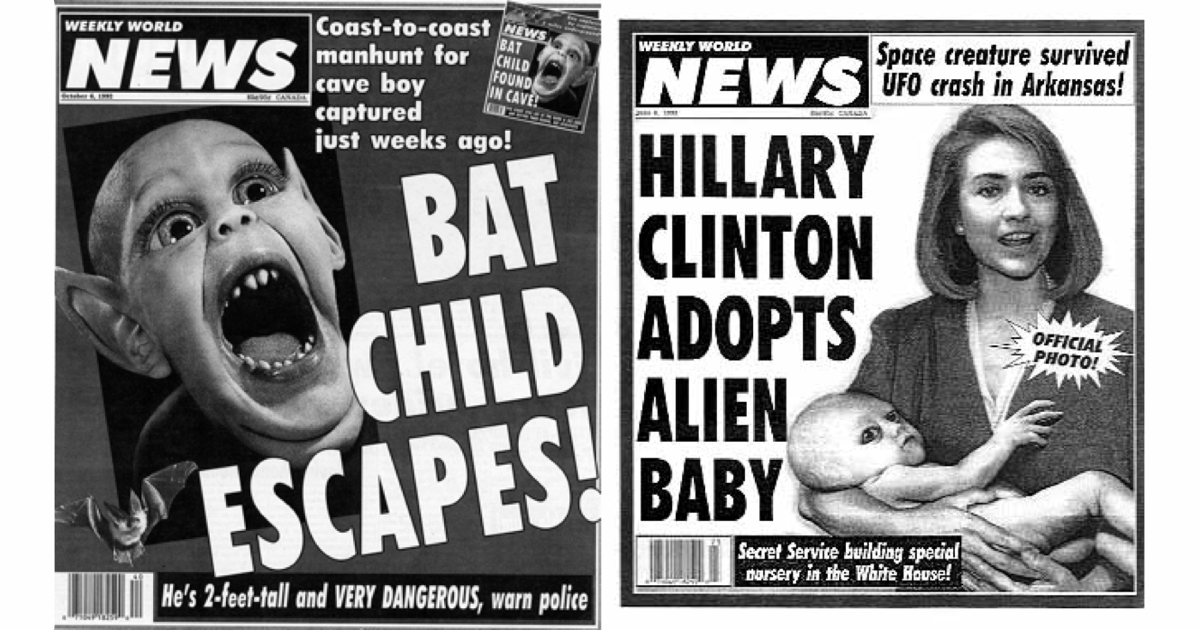
\includegraphics[width=25cm]{fake-news3.png}
\end{center}
\vfill

%%%%%%%%%%%%%%%%%%%%%%%%%%%%%%%%%%%%%%%%%%%%%%%%%%%%%%%%%%%%%%%%%%%%%%%%%%%%

\slide{Common Themes}
\vfill
\begin{itemize}
\item Hard problems $\rightarrow$ not solved, but {\em good enough} technology
\item Common methods with other subfields of artificial intelligence
\item Technology is advancing rapidly
\item New applications on (and just behind) horizon
\end{itemize}
\vfill

%%%%%%%%%%%%%%%%%%%%%%%%%%%%%%%%%%%%%%%%%%%%%%%%%%%%%%%%%%%%%%%%%%%%%%%%%%%%

\end{document}
